% $Header$

\documentclass[aspectratio=1610]{beamer}

\mode<presentation>
{%
  \usetheme{Boadilla}
}


\usepackage[english]{babel}
\usepackage[utf8]{inputenc}
\usepackage[T1]{fontenc}
\usepackage{%
    graphicx,
    varwidth,
    animate,
    tcolorbox,
    lmodern,
    clrscode3e,
}

\graphicspath{{../../imgs/}}

\newcommand{\alertline}{%
 \usebeamercolor[fg]{normal text}%
 \only{\usebeamercolor[fg]{alerted text}}}

\title[ALG25 - Lecture 2]
{Insertion sort \& Asymptotisk notation}

\subtitle
{Algorithms and Datastructures, F25, Lecture 2}

\author[Andreas H. Høeg-Petersen]
{Andreas Holck Høeg-Petersen}

\institute[AAU]{%
  Department of Computer Science\\
  Aalborg University
}

\date {\today}


% If you have a file called "university-logo-filename.xxx", where xxx
% is a graphic format that can be processed by latex or pdflatex,
% resp., then you can add a logo as follows:

\pgfdeclareimage[height=0.5cm]{university-logo}{../../imgs/aau-logo}
\logo{\pgfuseimage{university-logo}}

\AtBeginSection[]
{%
  \begin{frame}<beamer>{Outline}
    \tableofcontents[currentsection,currentsubsection]
  \end{frame}
}


\begin{document}

\begin{frame}
  \titlepage
\end{frame}

\begin{frame}{Opdateringer}{}
    \begin{itemize}
        \item Løsninger på exercises kommer på et eller andet tidspunkt
        \item Fra evaluering:
            \begin{itemize}
                \item Grupper?
                \item Andet?
            \end{itemize}
    \end{itemize}
\end{frame}


\begin{frame}{Outline}
  \tableofcontents
\end{frame}


\section{Insertion Sort}

\begin{frame}{Sorteringsproblemet}{En klassiker}
    \begin{description}
        \item[Input] En sekvens $A$ af $n$ tal $(a_1, a_2, \ldots, a_n)$
        \item[Output] En permutation $(a_1', a_2', \ldots, a_n')$ af $A$ således
            at $a_1' \leq a_2', \leq, \ldots, \leq a_n'$ \pause
    \end{description}

    \begin{itemize}[<+->]
        \item Tallene vi sorterer kalder vi også \alert{nøgler} (\textit{keys})
            \begin{itemize}
                \item Nøglerne er nogle gange forskellig fra den data, vi
                    egentlig sorterer
                \item F.eks.\ kunne vi sortere brugere (\alert{sattelit data})
                    på baggrund af deres alder (\alert{nøgler})
            \end{itemize}
        \item Sortering er tit et underproblem for mange andre problemer, der
            kan gøres nemmere ved først at sortere inputtet
        \item Der findes \underline{mange} sorteringsalgoritmer: merge sort,
            quicksort, bubble sort, heapsort, cocktail shaker sort, etc\ldots
    \end{itemize}

\end{frame}

\begin{frame}{Sorteringsproblemet}{En klassiker}
    \begin{figure}[h]
        \centering
        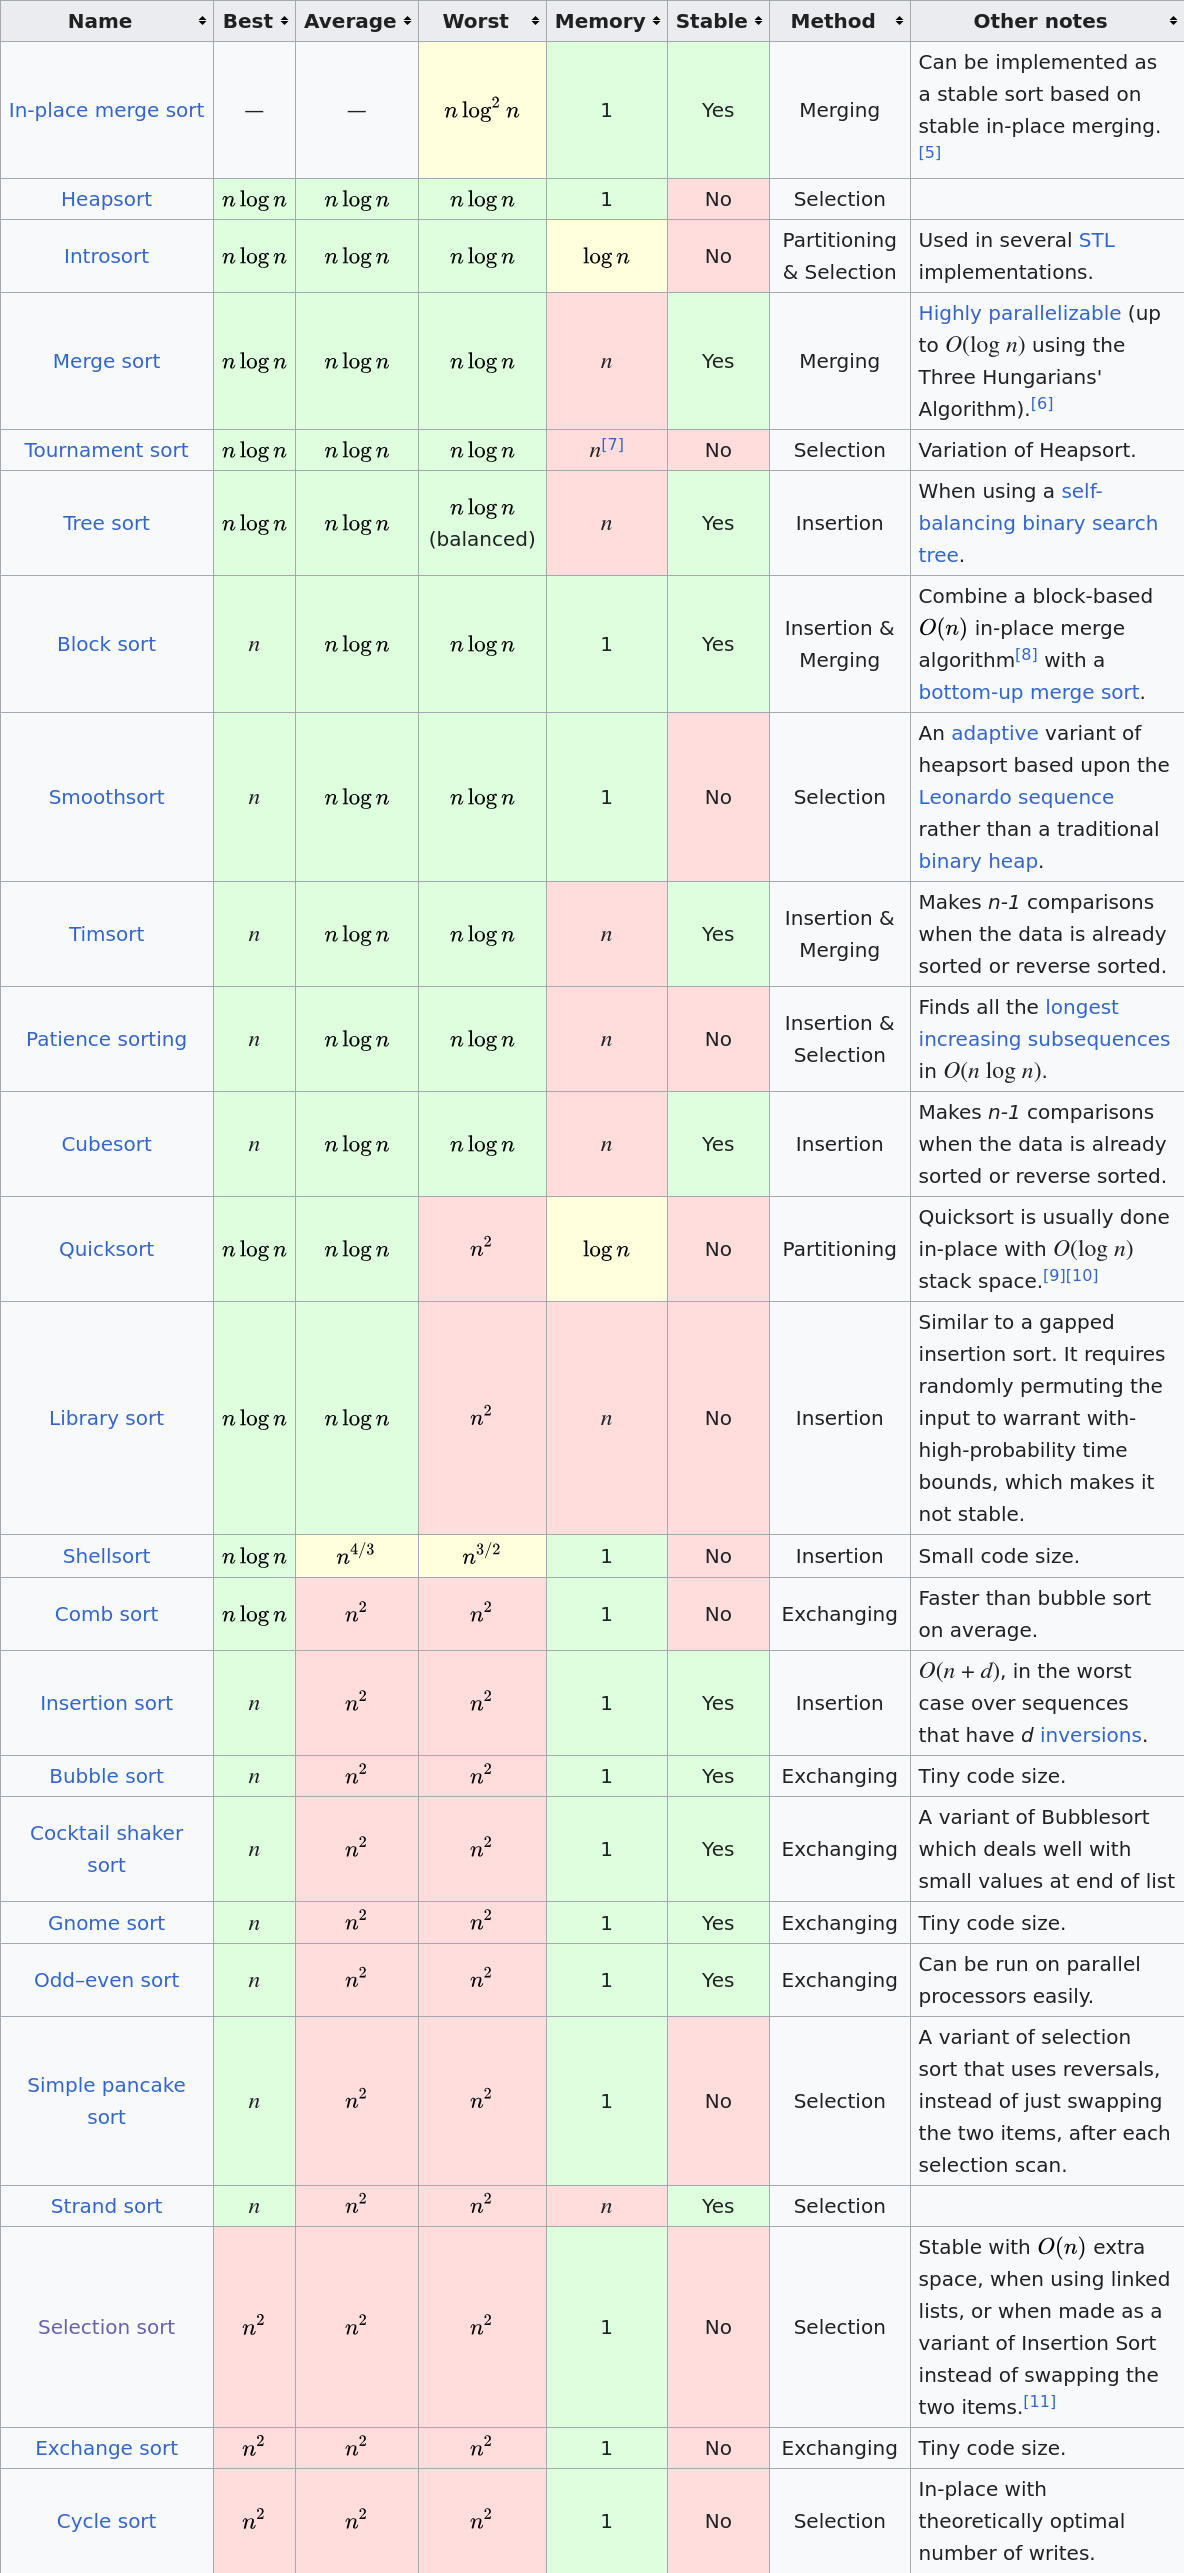
\includegraphics[width=0.21\textwidth]{sorting-algorithms-wiki}
        \caption{Screenshot fra Wikipedia}
        \label{fig:sorting-algorithms-wiki}
    \end{figure}
\end{frame}

\begin{frame}{Insertion sort}{Vores første sorteringsalgoritme!}
    \begin{itemize}
        \item Vi starter med at kigge på \alert{Insertion sort}
        \item Simple sorteringsalgoritme, effektiv for små værdier af $n$
            \begin{itemize}
                \item Hvad mener jeg med $n$?
                \item Også effektiv for \alert{næsten sorterede} sekvenser!
            \end{itemize}
        \item Kan ligne sortering af kort:
            \begin{itemize}
                \item Start med en tom hånd, kortbunken ligger på bordet
                \item Tag et kort af gangen fra bunken
                \item Søg i hånden til vi finder den korrekte position (fra
                    højre til venstre)
                \item Indsæt kortet på denne position
            \end{itemize}
    \end{itemize}
\end{frame}

\begin{frame}{Insertion-Sort}{Pseudo-kode}
    \centering
    \begin{minipage}{.8\textwidth}
        \begin{block}{Insertion-Sort($A$)}

        \vspace{-\abovedisplayskip}
            \begin{codebox}
                \li \For $i \gets 2$ \To $n$ \Do
                    \li $\id{key} \gets A[i]$
                    \li \Comment Insert $A[i]$ into the sorted sequence $A[1:i-1]$
                    \li $j \gets i - 1$
                    \li \While $j > 0$ and $A[j] > \id{key}$ \Do
                        \li $A[j+1] \gets A[j]$
                        \li $j \gets j - 1$
                    \End
                    \li $A[j+1] \gets \id{key}$
                \End
            \end{codebox}
        \end{block}
    \end{minipage}
    
\end{frame}



\begin{frame}[fragile]{Insertion sort}{Pseudo-kode}
    \begin{columns}

        \column{.5\textwidth}
        \begin{itemize}
            \small
            \only<1>{%
            \item Algoritmen tager et array $A[1:n]$ som input
            \item Vedligeholder to sub-arrays
                \begin{itemize}
                    \small
                    \item $A[1:i-1]$ er `kortene på hånden' (altid sorteret)
                    \item $A[i:n]$ er `kortene på bordet'
                \end{itemize}
            }

            \only<2->{%
            \item \alert<2>{Algoritmen gør 3 ting i hver iteration:}
                \begin{itemize}
                    \small
                    \item \alert<3>{Find det element $\id{key}$, der skal placeres korrekt
                        (i `hånden')}
                    \item \alert<4>{Gør plads i det sorterede sub-array (`hånden') ved at
                        flytte større elementer en plads bagud}
                    \item \alert<5>{Indsæt \id{key} på sin plads}
                \end{itemize}
            }
        \end{itemize}

        \column{.45\textwidth}

        \begin{minipage}{\textwidth}%
            \small

            \vspace{-\abovedisplayskip}
            \begin{codebox}
                \Procname{$\proc{Insertion-Sort}(A)$}
                \li \alertline<2>\For $i \gets 2$ \To $n$ \Do
                    \li \alertline<3>$\id{key} \gets A[i]$
                    \li \alertline<4>$j \gets i - 1$
                    \li \alertline<4>\While $j > 0$ and $A[j] > \id{key}$ \Do
                        \li \alertline<4>$A[j+1] \gets A[j]$
                        \li \alertline<4>$j \gets j - 1$
                    \End
                    \li \alertline<5>$A[j+1] \gets \id{key}$
                \End
            \end{codebox}
            
        \end{minipage}

    \end{columns}

\end{frame}

\begin{frame}[fragile]{Insertion sort}{Eksempel}
    \pause
    \begin{columns}

        \column{.45\textwidth}
        \begin{figure}[h]
            \centering
            \uncover<2->{%
                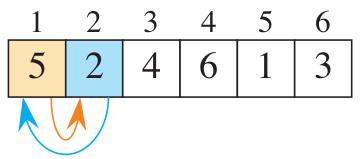
\includegraphics[width=0.4\textwidth]{insertion-sort-example/iter1}
            }
            \uncover<3->{%
                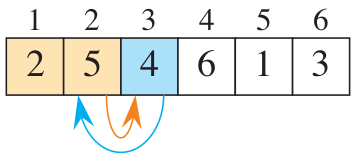
\includegraphics[width=0.4\textwidth]{insertion-sort-example/iter2}
            }
            \uncover<4->{%
                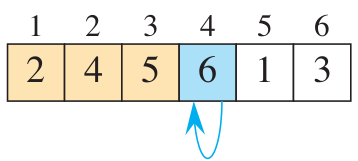
\includegraphics[width=0.4\textwidth]{insertion-sort-example/iter3}
            }
            \uncover<5->{%
                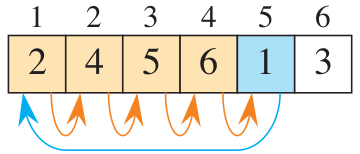
\includegraphics[width=0.4\textwidth]{insertion-sort-example/iter4}
            }
            \uncover<6->{%
                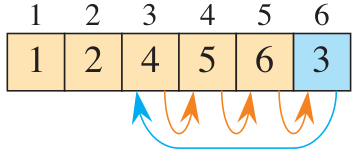
\includegraphics[width=0.4\textwidth]{insertion-sort-example/iter5}
            }
            \uncover<7->{%
                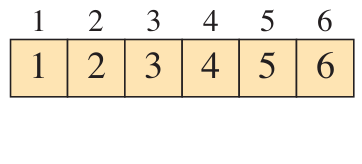
\includegraphics[width=0.4\textwidth]{insertion-sort-example/iter6}
            }
            \caption{Insertion sort example on input $[5,2,4,6,1,3]$}
            \label{fig:insertion-sort-example-iter6}
        \end{figure}

        \column{.45\textwidth}

        \begin{minipage}{\textwidth}%
            \small

            \vspace{-\abovedisplayskip}
            \begin{codebox}
                \Procname{$\proc{Insertion-Sort}(A)$}
                \li \For $i \gets 2$ \To $n$ \Do
                    \li $\id{key} \gets A[i]$
                    \li $j \gets i - 1$
                    \li \While $j > 0$ and $A[j] > \id{key}$ \Do
                        \li $A[j+1] \gets A[j]$
                        \li $j \gets j - 1$
                    \End
                    \li $A[j+1] \gets \id{key}$
                \End
            \end{codebox}
            
        \end{minipage}

    \end{columns}

\end{frame}

\begin{frame}{Insertion sort}{GIF!}
    \centering
    \animategraphics[loop,autoplay,width=4cm]{10}{insertion-sort-gif/insertion-sort-gif-}{0}{100}
\end{frame}

\section{Loop invarianter og korrekthed}

\begin{frame}{Loop invarianter}{Introduktion}
    Når vi ser på algoritmer skal vi gerne kunne argumentere for, at algoritmen
    faktisk virker --- og endnu bedre, vi skal gerne kunne \alert{bevise} det!
    En type korrekthedsbevis er ved hjælp af \alert{loop invarianter}.

    \begin{itemize}[<+->]
        \item En \alert{invariant} er en egenskab, der \textit{ikke} varierer;
            altså altid er sand
        \item Vi leder efter en egenskab, der relaterer sig til algoritmens
            opgave
        \item Vi vil så gerne vise, at
            \begin{itemize}
                \item Invarianten er sand når vi starter den første iteration
                    (\alert{initialization})
                \item Hvis den er sand, når en iteration starter, er den også
                    sand, når iterationen slutter (\alert{maintenance})
                \item Loopet terminerer på et tidspunkt, og invariantens
                    egenskab kan nu bruges til at vise algoritmens korrekthed
            \end{itemize}
    \end{itemize}
\end{frame}

\begin{frame}[fragile]{Loop invarianter}{Insertion sort}
    \pause
    \begin{columns}

        \column{.5\textwidth}
        \only<2-5>{%
            \textbf{Initialization}
            \begin{itemize}[<+->]
                \small
                \item Før den første iteration er $i=2$
                \item Sub-arrayet $A[1:i-1]$ består kun af et element $A[1]$
                \item Dette element er det samme, som oprindeligt var i $A[1]$ (for
                    vi har ikke ændret noget)
                \item Et array med kun 1 element er per definition sorteret
            \end{itemize}
        }

        \only<6-9>{%
            \textbf{Maintenance}
            \begin{itemize}
                \small
                \uncover<6->{%
                \item While-løkken flytter \alert{et} element fra $A[i]$ til
                    dets korrekte plads i $A[1:i]$
                }
                \uncover<7->{%
                \item Sub-arrayet indeholder nu stadig de oprindelige elementer
                    fra $A[1:i]$, stadig i sorteret orden
                }
                \uncover<8->{%
                \item Når vi inkrementerer $i$ opretholdes loop-invarianten
                }
                \uncover<9->{%
                \item NB: I teorien burde vi have lavet samme øvelse for
                    while-løkken selv, men\ldots
                }
            \end{itemize}
        }

        \only<10->{%
            \textbf{Termination}
            \begin{itemize}
                \small
                \uncover<10->{%
                \item For-løkken stopper når $i$ er større end $n$. Da $i$
                    starter ved 2 og inkrementeres i hver iteration, vil løkken
                    terminere når $i = n + 1$
                }
                \uncover<11->{%
                \item Indsætter vi $n+1$ i loop-invarianten får vi $A[1:(n+1)-1]
                    = A[1:n]$
                }
                \uncover<12->{%
                \item Altså får vi, at $A[1:n]$ indeholder alle de oprindelige
                    elementer, men nu i sorteret rækkefølge
                }
                \uncover<13->{%
                \item Eftersom $A[1:n]$ er hele arrayet, kan vi konkludere, at
                    $A$ er sorteret og algoritmen er \alert{korrekt}
                }
            \end{itemize}
        }

        \column{.45\textwidth}

        \begin{minipage}{\textwidth}%
            \small

            \vspace{-\abovedisplayskip}
            \begin{codebox}
                \Procname{$\proc{Insertion-Sort}(A)$}
                \li \For $i \gets 2$ \To $n$ \Do
                    \li $\id{key} \gets A[i]$
                    \li $j \gets i - 1$
                    \li \While $j > 0$ and $A[j] > \id{key}$ \Do
                        \li $A[j+1] \gets A[j]$
                        \li $j \gets j - 1$
                    \End
                    \li $A[j+1] \gets \id{key}$
                \End
            \end{codebox}
            
        \end{minipage}

    \end{columns}

    \begin{block}{Loop invariant}
        Ved begyndelse af hver iteration af \alert{for-løkken} består
        sub-arrayet $A[1:i-1]$ af de oprindelige elementer i $A[1:i-1]$ men i
        sorteret rækkefølge.
    \end{block}

\end{frame}

\section{Exercises}

\begin{frame}{Exercises!}{Yay!}
    
    \begin{figure}[h]
        \centering
        
\includegraphics[width=0.8\textwidth]{exercises}
    \end{figure}
    
\end{frame}


\section{Asymptotisk notation og analyse}

\begin{frame}{Tidskompleksitet}{Recap}
    Vi så i sidste uge, hvordan vi i lidt grove træk kan angive køretiden på en
    algoritme. Lad os prøve på \proc{Insertion-Sort}! Vi siger, at while-løkken
    kører $t_i$ gange for en eller anden værdi af $i$:

    \begin{columns}
        \column{.5\textwidth}
        \begin{codebox}
            \Procname{$\proc{Insertion-Sort}(A)$}
            \li \For $i \gets 2$ \To $n$ \Do
                \li $\id{key} \gets A[i]$
                \li $j \gets i - 1$
                \li \While $j > 0$ and $A[j] > \id{key}$ \Do
                    \li $A[j+1] \gets A[j]$
                    \li $j \gets j - 1$
                \End
                \li $A[j+1] \gets \id{key}$
            \End
        \end{codebox}
        
        \column{.5\textwidth}
        \begin{codebox}
            \Procname{tid $\times$ antal gange}
            \zi \uncover<2->{{$c_1 \times n$}}
            \zi \uncover<3->{{$c_2 \times n - 1$}}
            \zi \uncover<4->{{$c_3 \times n - 1$}}
            \zi \uncover<5->{{$c_4 \times \sum^{n}_{i=2}t_i$}}
            \zi \uncover<6->{{$c_5 \times \sum^{n}_{i=2}(t_i-1)$}}
            \zi \uncover<7->{{$c_6 \times \sum^{n}_{i=2}(t_i-1)$}}
            \zi \uncover<8->{{$c_7 \times n - 1$}}
        \end{codebox}
    \end{columns}

    \medskip
    \uncover<9>{%
        Hmm\ldots Hvad er best case? Hvad er worst case?
    }

\end{frame}

\begin{frame}{Tidskompleksitet}{Recap}
    \begin{description}
        \uncover<2->{%
            \item[Best case] $A$ er allerede sorteret, og vi kommer aldrig ind i
                while-løkken $\Rightarrow t_i = 0$ for alle $i = 2\ldots n$
        }
        \uncover<3->{%
            \item[Worst case] $A$ er omvendt sorteret, og vi skal helt i bund
                hver gang $\Rightarrow t_i = i$ for alle $i = 2\ldots n$
        }
    \end{description}

    \begin{columns}
        \column{.5\textwidth}
        \begin{codebox}
            \Procname{$\proc{Insertion-Sort}(A)$}
            \li \For $i \gets 2$ \To $n$ \Do
                \li $\id{key} \gets A[i]$
                \li $j \gets i - 1$
                \li \While $j > 0$ and $A[j] > \id{key}$ \Do
                    \li $A[j+1] \gets A[j]$
                    \li $j \gets j - 1$
                \End
                \li $A[j+1] \gets \id{key}$
            \End
        \end{codebox}
        
        \column{.5\textwidth}
        \begin{codebox}
            \Procname{tid $\times$ antal gange}
            \zi $c_1 \times n$
            \zi $c_2 \times n - 1$
            \zi $c_3 \times n - 1$
            \zi $c_4 \times \only<1>{\sum^{n}_{i=2}t_i}
                    \only<2>{n-1}
                    \only<3>{\sum^{n}_{i=2}i}
                    \only<4->{\frac{n(n+1)}{2}-1}$
            \zi $c_5 \times \only<1>{\sum^{n}_{i=2}(t_i-1)}
                    \only<2>{0}
                    \only<3>{\sum^{n}_{i=2}(i-1)}
                    \only<4->{\frac{n(n-1)}{2}}$
            \zi $c_6 \times \only<1>{\sum^{n}_{i=2}(t_i-1)}
                    \only<2>{0}
                    \only<3>{\sum^{n}_{i=2}(i-1)}
                    \only<4->{\frac{n(n-1)}{2}}$
            \zi $c_7 \times n - 1$
        \end{codebox}
    \end{columns}

\end{frame}

\begin{frame}{Tidskompleksitet}{Recap}
    Og husk, vi er primært interessert i worst case. Men det efterlader os så
    med\ldots

    \begin{align*}
        T(N) =& c_1n + c_2(n-1) + c_3(n-1) + c_4\left(\frac{n(n+1)}{2}-1\right) \\
              &+ c_5 \left(\frac{n(n-1)}{2}\right) +
              c_6 \left(\frac{n(n-1)}{2}\right) + c_7(n-1) \\
        \uncover<2->{%
        =& \left(\frac{c_4}{2} + \frac{c_5}{2} + \frac{c_6}{2}\right)n^2 + 
        \left(c_1 + c_2 + c_3 + \frac{c_4}{2} - \frac{c_5}{2} -
            \frac{c_6}{2} + c_7\right)n \\
         &- (c_2 + c_3 + c_4 + c_7) \\
         }
         \uncover<3->{%
        =& an^2 + bn + c
        }
    \end{align*}
\end{frame}

\begin{frame}{Asymptotisk analyse}{Order of growth}
    Det leder os videre til en ny måde at tale om kompleksitet på, nemlig i
    termer af \alert{order of growth}.

    \begin{itemize}
        \item Den eksakte køretid er sjældent særligt relevant --- vi vil
            hellere abstrahere
        \item For små inputs er køretiden også irrelevant (computere er
            hurtige!)
        \item For store inputs er konstanter og små termer irrelevante --- det
            essentielle er, hvordan køretiden \alert{udvikler sig} som en funktion
            af $n$
        \item Vi studerer derfor \alert{asymptotisk køretid}
            \begin{itemize}
                \item Hvordan vokser køretiden, når inputtet bliver større?
            \end{itemize}
    \end{itemize}
\end{frame}

\begin{frame}{Asymptotisk notation}{Big-Oh, Big-Omega, Big-Theta}
    Målet med asymptotisk analyse er forenkle udtrykket for køretiden ved at
    abstrahere irrelevante og svært forudsigelige faktorer væk og istedet fange
    `essensen' af $T(n)$ --- nemlig den dominerende term, når $n$ går mod
    $\infty$.

    \pause
    \medskip

    Vi har 3 notationer, vi bruger:

    \begin{description}[Big-Omega, $\Omega$]
        \item[Big-Oh, $O$] Asymptotisk \alert{upper bound}
        \item[Big-Omega, $\Omega$] Asymptotisk \alert{lower bound}
        \item[Big-Theta, $\Theta$] Asymptotisk \alert{thight bound}
    \end{description}

    Både $O, \Omega$ og $\Theta$ definerer \alert{sæt af funktioner}, som en
    funktion for tidskompleksiteten kan høre til.
\end{frame}

\begin{frame}{Asymptotisk notation}{Big-Oh}
    \begin{definition}[Big-Oh, $O$]
        For en given funktion $g(n)$ er $O(g(n))$ det sæt af funktioner, således
        at

        \vspace{-\abovedisplayskip}
        \begin{align*}
            O(g(n)){} =&\{ f(n) : \text{der eksisterer positive konstanter } c
                \text{~og~} n_0 \\
                       &\text{~sådan at~} 0 \leq f(n) \leq cg(n) \text{~for
                   alle~} n \geq n_0 \}
        \end{align*}
    \end{definition}

    \pause
    \begin{columns}
        \column{.6\textwidth}
        \begin{itemize}[<+->]
            \small
            \item Vi skriver $T(n) = O(g(n))$ hvis $T(n) \in O(g(n))$ 
            \item Intuition: $T(n)$ vokser asymptotisk langsommere end $g(n)$
            \item Eksempler:
                \begin{itemize}
                    \tiny
                    \item $T(n) = 23n^3 + 1000n = O(n^3)$
                    \item $T(n) = 23n^3 + 1000n = O(n^4)$
                    \item $T(n) = 2^n + 41n^27 = O(2^n)$
                    \item $T(n) = 100 = O(1)$
                \end{itemize}
        \end{itemize}

        \column{.4\textwidth}

        \begin{figure}[h]
            \centering
            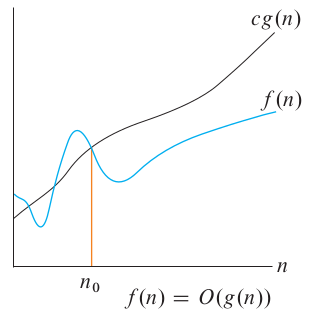
\includegraphics[width=0.7\textwidth]{asymptotic-notation/big-oh}
        \end{figure}

    \end{columns}
\end{frame}

\begin{frame}{Asymptotisk notation}{Big-Oh}
    \begin{definition}[Big-Oh, $O$]
        For en given funktion $g(n)$ er $O(g(n))$ det sæt af funktioner, således
        at

        \vspace{-\abovedisplayskip}
        \begin{align*}
            O(g(n)){} =&\{ f(n) : \text{der eksisterer positive konstanter } c
                \text{~og~} n_0 \\
                       &\text{~sådan at~} 0 \leq f(n) \leq cg(n) \text{~for
                   alle~} n \geq n_0 \}
        \end{align*}
    \end{definition}

    Eksempel:
    \pause
    \begin{itemize}[<+->]
        \small
        \item Vi vil vise, at funktionen $f(n) = n^2 + 1000n + 500 = O(n^2)$
        \item Vi skal dermed finde $c$ og $n_0$ således, at $n^2 + 1000n + 500
            \leq cn^2$ for all $n \geq n_0$
        \item Vi dividerer begge sider med $n^2$, hvilket giver $1 + 1000/n +
            500/n^2 \leq c$
        \item Her skulle det være nemt at se, at jo større $n_0$, jo mindre et $c$
            kan vi klare os med --- f.eks.\ ved $n_0 = 2$ bliver venstresiden af
            uligheden 629, og vi kan vælge et hvilket som helst $c \geq 629$.
            Hvis vi vælger $n_0 = 100$ kan vi vælge et $c \geq 11.05$
    \end{itemize}
\end{frame}


\begin{frame}{Asymptotisk notation}{Big-Omega}
    \begin{definition}[Big-Omega, $\Omega$]
        For en given funktion $g(n)$ er $\Omega(g(n))$ det sæt af funktioner,
        således at

        \vspace{-\abovedisplayskip}
        \begin{align*}
            \Omega(g(n)){} =&\{ f(n) : \text{der eksisterer positive
                konstanter~} c \text{~og~} n_0 \\
                       &\text{~sådan at~} 0 \leq cg(n) \leq f(n) \text{~for
                   alle~} n \geq n_0 \}
        \end{align*}
    \end{definition}

    \pause
    \begin{columns}
        \column{.6\textwidth}
        \begin{itemize}[<+->]
            \small
            \item Vi skriver $T(n) = \Omega(g(n))$ hvis $T(n) \in \Omega(g(n))$ 
            \item Intuition: $T(n)$ vokser asymptotisk hurtigere end $g(n)$
            \item Eksempler:
                \begin{itemize}
                    \tiny
                    \item $T(n) = 23n^3 + 1000n = \Omega(n^3)$
                    \item $T(n) = 23n^3 + 1000n = \Omega(n)$
                    \item $T(n) = 2^n + 41n^{27} = \Omega(2^n)$
                    \item $T(n) = 100 = \Omega(1)$
                \end{itemize}
        \end{itemize}

        \column{.4\textwidth}

        \begin{figure}[h]
            \centering
            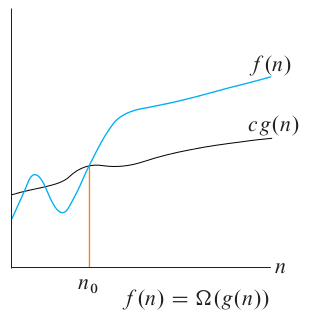
\includegraphics[width=0.7\textwidth]{asymptotic-notation/big-omega}
        \end{figure}

    \end{columns}
\end{frame}

\begin{frame}{Asymptotisk notation}{Big-Theta}
    \begin{definition}[Big-Theta, $\Theta$]
        For en given funktion $g(n)$ er $\Theta(g(n))$ det sæt af funktioner,
        således at

        \vspace{-\abovedisplayskip}
        \begin{align*}
            \Theta(g(n)){} =&\{ f(n) : \text{der eksisterer positive konstanter~}
                c_1, c_2 \text{~og~} n_0 \\
                       &\text{~sådan at~} 0 \leq c_1g(n) \leq f(n) \leq c_2g(n)
                   \text{~for alle~} n \geq n_0 \}
        \end{align*}
    \end{definition}

    \pause
    \begin{columns}
        \column{.6\textwidth}
        \begin{itemize}[<+->]
            \small
            \item Intuition: $g(n)$ er et asymptotisk tight bound for $T(n)$
            \item Theorem: for to funktioner $f(n)$ og $g(n)$ har vi at $f(n) =
                \Theta(g(n))$ hvis og kun hvis $f(n) = \Omega(g(n))$ og $f(n) =
                O(g(n))$
            \item Eksempler:
                \begin{itemize}
                    \tiny
                    \item $T(n) = 23n^3 + 1000n = \Theta(n^3)$
                    \item $T(n) = 2^n + 41n^{27} = \Theta(2^n)$
                    \item $T(n) = 100 = \Theta(1)$
                \end{itemize}
        \end{itemize}

        \column{.4\textwidth}

        \begin{figure}[h]
            \centering
            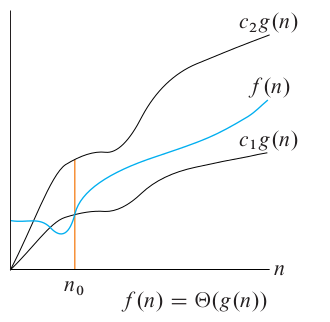
\includegraphics[width=0.7\textwidth]{asymptotic-notation/big-theta}
        \end{figure}

    \end{columns}
\end{frame}

\begin{frame}{Asymptotisk notation}{Tips og tricks}

    Denne nemme måde (`ingeniørmetoden') til at bruge asymptotisk notation:
    \pause
    \begin{itemize}[<+->]
        \item Ignorer indledende konstanter
            \begin{itemize}
                \item $T(n) = 1000n^2 = \Theta(n^2)$
            \end{itemize}
        \item Ignorer mindre termer
            \begin{itemize}
                \item $T(n) = n^3 + 1000n^2 - n \log n + 13n = \Theta(n^3)$
            \end{itemize}
        \item Hvordan identificerer man mindre termer?
            \begin{itemize}
                \item $c < \log n < n < n \log n < n^a < b^n < n!~$
                \item Konstant, logaritmisk, log linear, polynomial,
                    eksponentiel, fakultet
            \end{itemize}
    \end{itemize}

    \pause
    \begin{figure}[h]
        \centering
        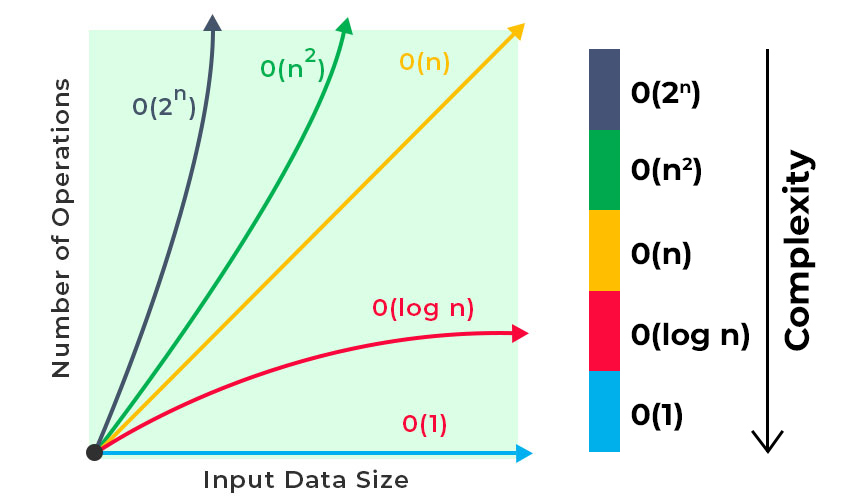
\includegraphics[width=0.38\textwidth]{time-complexity}
        \caption{Source: https://www.geeksforgeeks.org/what-is-logarithmic-time-complexity/}
        \label{fig:time-complexity}
    \end{figure}
\end{frame}

\begin{frame}{Asymptotisk analyse}{Insertion sort}

    Vi slutter, hvor vi startede --- med Insertion-Sort. Nu da vi kender til
    asymptotisk analyse og notation, kan vi så gribe vores analyse lidt lettere
    an?

    \begin{columns}
        \column{.5\textwidth}
        \begin{codebox}
            \small
            \Procname{$\proc{Insertion-Sort}(A)$}
            \li \alertline<2> \For $i \gets 2$ \To $n$ \Do
                \li $\id{key} \gets A[i]$
                \li $j \gets i - 1$
                \li \alertline<3>\While $j > 0$ and $A[j] > \id{key}$ \Do
                    \li \alertline<3>$A[j+1] \gets A[j]$
                    \li \alertline<3>$j \gets j - 1$
                \End
                \li $A[j+1] \gets \id{key}$
            \End
        \end{codebox}
        
        \column{.5\textwidth}
        
        \pause
        \begin{itemize}[<+->]
            \small
            \item Vi ser, at hele algoritmen er pakket ind i en for-løkke, der kører
                $\Theta(n)$ gange
            \item Vi ser, at der i for-løkken er en while-løkke, der i worst case
                selv kører $\Theta(n)$ gange
            \item Resten af linierne er konstanter, altså har vi $T(n) = \Theta(n)
                \cdot \Theta(n) = \Theta(n^2)$
        \end{itemize}

    \end{columns}

\end{frame}

\begin{frame}{Dagens temaer}{Opsummering}
    \begin{itemize}
        \item Vi har mødt vores første sorteringsalgoritme --- Insertion-Sort!
            \begin{itemize}
                \item Simpel at implementere og forstå
                \item God til næsten sorterede sekvenser
                \item Den asymptotiske worst case køretid er kvadratisk
            \end{itemize}
        \item Loop invarianter og korrekthed
            \begin{itemize}
                \item Initialization, maintenance og termination
            \end{itemize}
        \item Asymptotisk analyse og notation
            \begin{itemize}
                \item $O, \Omega, \Theta$
            \end{itemize}
    \end{itemize}
\end{frame}


\begin{frame}{Tak for i dag!}{Flere exercises..}

    Den bedste måde ikke at snyde sig selv på er lave exercises!

    \begin{figure}[h]
        \centering
        
\includegraphics[width=0.8\textwidth]{exercises}
    \end{figure}
    
\end{frame}



\end{document}


